\documentclass[12pt, titlepage]{article}

\usepackage{booktabs}
\usepackage{tabularx}
\usepackage{hyperref}
\usepackage{float}
\usepackage{graphicx}
\usepackage[letterpaper, portrait, margin=1in]{geometry}
\usepackage{helvet}
\hypersetup{
    colorlinks,
    citecolor=black,
    filecolor=black,
    linkcolor=red,
    urlcolor=blue
}
\usepackage[round]{natbib}
\graphicspath{ {./docs/VNVReport} }
\renewcommand{\familydefault}{\sfdefault}
%% Comments

\usepackage{color}

\newif\ifcomments\commentstrue %displays comments
%\newif\ifcomments\commentsfalse %so that comments do not display

\ifcomments
\newcommand{\authornote}[3]{\textcolor{#1}{[#3 ---#2]}}
\newcommand{\todo}[1]{\textcolor{red}{[TODO: #1]}}
\else
\newcommand{\authornote}[3]{}
\newcommand{\todo}[1]{}
\fi

\newcommand{\wss}[1]{\authornote{blue}{SS}{#1}} 
\newcommand{\plt}[1]{\authornote{magenta}{TPLT}{#1}} %For explanation of the template
\newcommand{\an}[1]{\authornote{cyan}{Author}{#1}}

%% Common Parts

\newcommand{\progname}{ProgName} % PUT YOUR PROGRAM NAME HERE
\newcommand{\authname}{Team \#, Team Name
\\ Student 1 name and macid
\\ Student 2 name and macid
\\ Student 3 name and macid
\\ Student 4 name and macid} % AUTHOR NAMES                  

\usepackage{hyperref}
    \hypersetup{colorlinks=true, linkcolor=blue, citecolor=blue, filecolor=blue,
                urlcolor=blue, unicode=false}
    \urlstyle{same}
                                


\begin{document}

\title{Verification and Validation Report: \progname} 
\author{\authname}
\date{\today}
	
\maketitle

\pagenumbering{roman}

\section{Revision History}

\begin{tabularx}{\textwidth}{p{3cm}p{2cm}X}
\toprule {\bf Date} & {\bf Version} & {\bf Notes}\\
\midrule
Date 1 & 1.0 & Notes\\
Date 2 & 1.1 & Notes\\
\bottomrule
\end{tabularx}

~\newpage

\section{Symbols, Abbreviations and Acronyms}

\renewcommand{\arraystretch}{1.2}
\begin{tabular}{l l} 
  \toprule		
  \textbf{symbol} & \textbf{description}\\
  \midrule 
  T & Test\\
  \bottomrule
\end{tabular}\\

\wss{symbols, abbreviations or acronyms -- you can reference the SRS tables if needed}

\newpage

\tableofcontents

\listoftables %if appropriate

\listoffigures %if appropriate

\newpage

\pagenumbering{arabic}

This document ...

\section{Functional Requirements Evaluation}

\section{Nonfunctional Requirements Evaluation}

\subsection{Usability}
		
\subsection{Performance}

\subsection{etc.}
	
\section{Comparison to Existing Implementation}	

Current motion detecting smart watches, such as Apple watches or Samsung Galaxy watches, are desgined for healthy and active population. The EMAnator is specifically geared towards older adults who have chronical back pain. Therefore, it is desgined to capture minor and subtle movements accurately.

\section{Unit Testing}

\begin{center}
\begin{tabular}{ c | c | c | c | c | c | c | c }
 1 & Void bed\_HR\_setup() & Set-up function for heartrate module & RQ & User heart rate input from A0 signal pin. & "PulseSensor object created", LED flash & Actual & Pass \\ 
2 & name & desc & ref & input & expected & actual & pass or fail \\  
3 & name & desc & ref & input & expected & actual & pass or fail \\  
\end{tabular}
\end{center}

\section{Changes Due to Testing}

After testing out each unit of the device system and failing unit test \#2, the type of heartrate sensor has been changed. Now the ... (list out all the potential candidates that were ruled out).\\

\textbf{Heart Rate Sensor Options:}\\

\begin{table}[H]
\begin{tabular}{ | c | m{3cm} | c | m{7cm} |}
\hline
\textbf{Image} & \textbf{Model} & \textbf{Status} & \textbf{Reason for Status}\\
\hline
 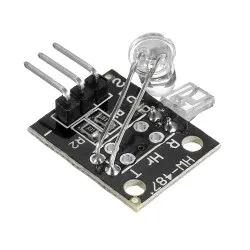
\includegraphics[scale = 0.5]{G21394} & \href{https://secure.sayal.com/STORE2/View_SHOP.php?SKU=247799}{Chaney Electronics Inc. G21394}  & Rejected & Due to the Infrared LED's Placement and the photoelectic sensor's placement, it is impossible to integrate the module with a device sitting on the wrist.\\
\hline
 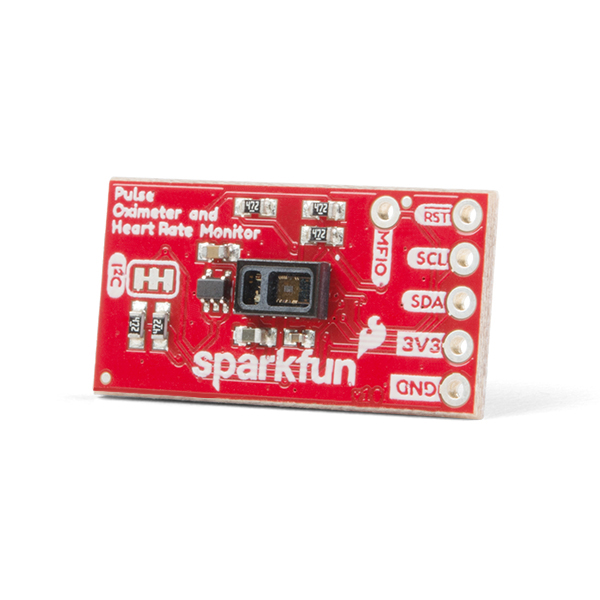
\includegraphics[scale = 0.5]{sparkfun} & \href{https://www.sparkfun.com/products/15219}{SparkFun Pulse Oximeter and Heart Rate Sensor - MAX30101 \& MAX32664 (Qwiic)}  & Rejected & Chronically out of stock, and requires extra complexity to be built into the PCB in order for this to function.\\
\hline
 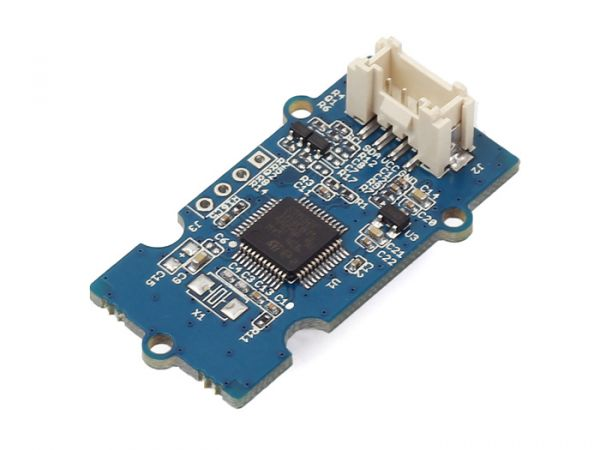
\includegraphics[scale = 0.25]{grove1} & \href{https://www.seeedstudio.com/Grove-Finger-clip-Heart-Rate-Sensor.html?queryID=ad9334e40c7058a87ffd810044eecd1c&objectID=711&indexName=bazaar_retailer_products}{Grove - Finger-clip Heart Rate Sensor}  & Rejected & Size too large, and issues with skin contact to the sensor results in garbage data.\\
\hline
 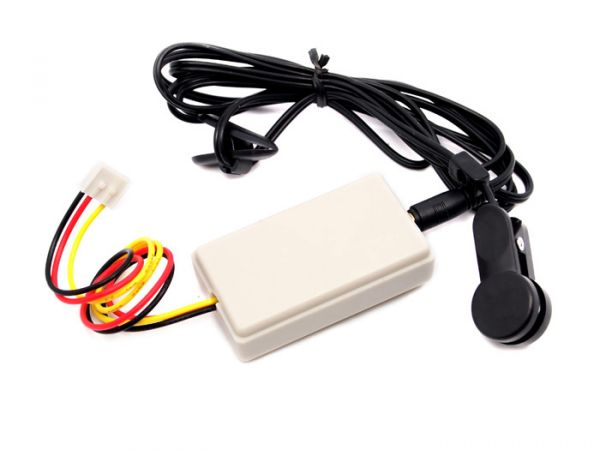
\includegraphics[scale = 0.25]{grove2} & \href{https://www.seeedstudio.com/Grove-Ear-clip-Heart-Rate-Sensor.html?queryID=ad9334e40c7058a87ffd810044eecd1c&objectID=2143&indexName=bazaar_retailer_products}{Grove - Ear-clip/Finger-clip Heart Rate Sensor}  & Rejected & Sensor attachment to the ear was considered too disruptive to the participant's daily activities.\\
\hline
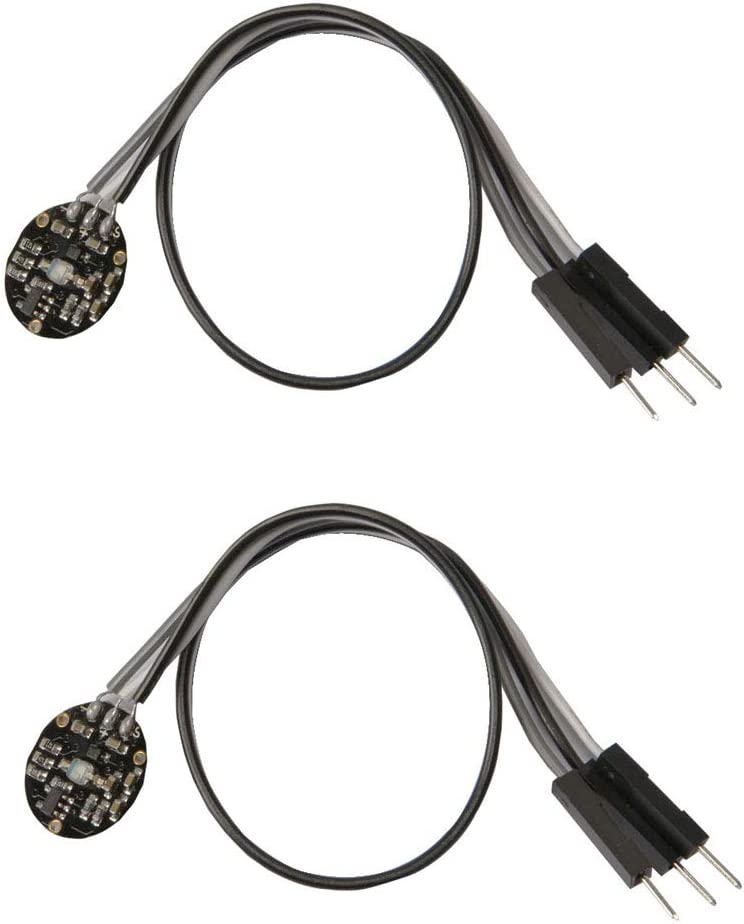
\includegraphics[scale = 0.1]{knockoff} & \href{https://www.amazon.ca/Comimark-Sensor-Module-Arduino-Raspberry/dp/B07V6VV8CM}{Comimark 2Pcs Heart Rate Pulse Sensor Sensor Module for Arduino Raspberry pi}  & Rejected & Build quality was unacceptably bad. Ordered name-brand version of this product next.\\
\hline

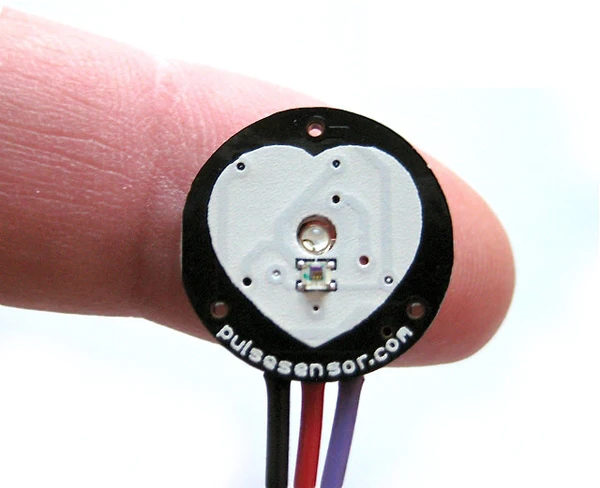
\includegraphics[scale = 0.25]{pulseSensor} & \href{https://pulsesensor.com/}{PulseSensor.com Pulse Sensor}  & Accepted & Build quality was better than knock-offs from before. Skin contact issue still present, but attempts are being made to solve this issue using software.\\
\hline
\end{tabular}
\end{table}

\section{Automated Testing}
N/A

\section{Trace to Requirements}
		
\section{Trace to Modules}		

\section{Code Coverage Metrics}

%\bibliographystyle{plainnat}
%\bibliography{../../refs/References}

\newpage{}
\section*{Appendix --- Reflection}

The information in this section will be used to evaluate the team members on the
graduate attribute of Reflection.  Please answer the following question:

\begin{enumerate}
  \item In what ways was the Verification and Validation (VnV) Plan different
  from the activities that were actually conducted for VnV?  If there were
  differences, what changes required the modification in the plan?  Why did
  these changes occur?  Would you be able to anticipate these changes in future
  projects?  If there weren't any differences, how was your team able to clearly
  predict a feasible amount of effort and the right tasks needed to build the
  evidence that demonstrates the required quality?  (It is expected that most
  teams will have had to deviate from their original VnV Plan.)
\end{enumerate}

\end{document}